\chapter{Definite Integrals}

Integrals are a fundamental concept in calculus, which are used to
calculate areas, volumes, and many other things. A definite integral
calculates the net area between the function and the x-axis over a
given interval.

Recall that you can use a Riemann sum to estimate the area under a function, and that as we increase the number of subintervals, the estimated area approaches the actual area. In sigma notation we can express a Riemann sum as $$\sum_{i=1}^{n} f(x_i)\Delta x$$

\section{Definition}

The definite integral of a function $f(x)$ over an interval $[a, b]$
is defined as the limit of a Riemann sum as $n$ approaches $\infty$:

\begin{equation}
\int_{a}^{b} f(x) \, dx = \lim_{{n \to \infty}} \sum_{i=1}^{n} f(x_i^*) \Delta x
\end{equation}

where $x_i^*$ is a sample point in the $i^{th}$ subinterval of a
partition of $[a, b]$, $\Delta x = \frac{b-a}{n}$ is the width of each
subinterval, and the limit is taken as the number of subintervals $n$
approaches infinity.

\begin{Exercise}[label=defint1]
Express $$\lim_{n \to \infty} \sum_{i=1}^{n} (x_i^3+x_i\sin{x_i})\Delta x$$ as an integral on the interval $[0, \pi]$. 
\end{Exercise}

\begin{Answer}[ref=defint1]
Following the structure shown in the formal definition of a definite integral, we can set $f(x) = x^3+x\sin{x}$ and re-write the limit of the sum as $\lim_{n \to \infty} \Sigma_{i=1}^{n} f(x)\Delta x=\int_{0}^{\pi} f(x) \, dx$. Therefore, the full definite integral would be written as $\int_{0}^{\pi} (x^3 + x\sin{x})\, dx$. 
\end{Answer}

\section{Positive and Negative Areas}
%explain when function is below graph, area is negative and so sum represents NET area

\section{Properties of Integrals}
The following properties of integrals apply when $f(x)$ is continuous or has a finite number of jump discontinuities on the interval $a \leq x \leq b$:
\begin{enumerate}
\item $$\int_{a}^{b}f(x)\, dx = -\int_{b}^{a}f(x)\, dx$$ %Property 1
\item If $a=b$, then $\Delta x = 0$ and therefore $$\int_{a}^{a}f(x)\, dx = 0$$%Property 2
\item $$\int_{a}^{b}c\,dx = c(b-a)\text{, where }c\text{ is any constant}$$%Property 3
\item $$\int_{a}^{b}[f(x) + g(x)]\,dx = \int_{a}^{b}f(x)\,dx + \int_{a}^{b}g(x)\,dx$$%Property 4
\item $$\int_{a}^{b}cf(x)\,dx = c\int_{a}^{b}f(x)\text{, where }c\text{ is any constant}$$%Property 5
\item $$\int_{a}^{b}[f(x) - g(x)]\,dx = \int_{a}^{b}f(x)\,dx - \int_{a}^{b}g(x)\,dx$$%Property 6
\item $$\int_{a}^{c} f(x)\,dx + \int_{c}^{b}f(x)\,dx = \int_{a}^{b}f(x)\,dx\text{, where }a<c<b$$%Property 7
\item $$\text{If }f(x) \geq 0\text{ for }a\leq x\leq b\text{, then }\int_{a}^{b}f(x)\,dx \geq0$$%Property 8
\item $$\text{If }f(x)\geq g(x)\text{ for }a\leq x \leq b\text{, then}\int_{a}^{b}f(x)\,dx \geq \int_{a}^{b}g(x)\,dx$$%Property 9
\item $$\text{If } m \leq f(x) \leq M\text{ for }a\leq x \leq b\text{, then }m(b-a)\leq \int_{a}^{b}f(x)\,dx \leq M(b-a)$$%Property 10
\end{enumerate}


\section{Applications in Physics}
We've already seen that the area under a velocity function is displacement and the area under an acceleration function is change in velocity (Riemann Sums). We can use integrals to determine the change in position of an object over a given time frame. If we \textit{also} know the object's starting position, then we can state the object's ending position. Consider the graph of an object's velocity in figure \ref{fig:velocity}:

\begin{figure}[htbp]
	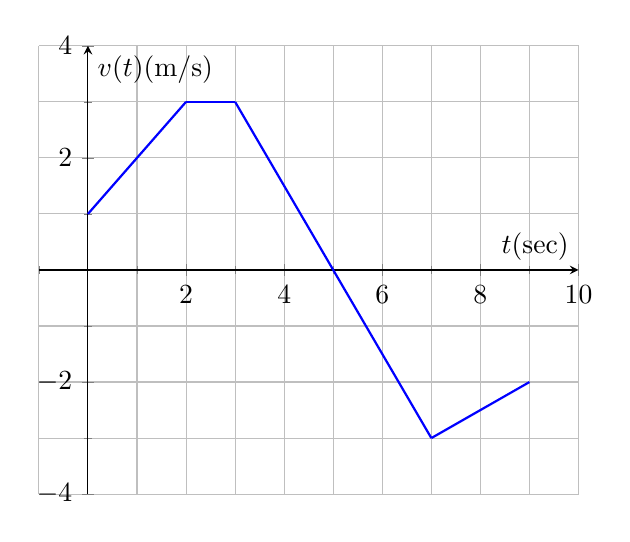
\begin{tikzpicture}
		\begin{axis}[axis lines = center, xmin=-1, xmax=10, ymin=-4, ymax=4, xlabel=$t$(sec), ylabel=$v(t)$(m/s), xtick={}, ytick={}, grid=both, minor tick num = 1]
		\addplot[blue, thick] coordinates {(0, 1) (2, 3)};
		\addplot[blue, thick] coordinates {(2, 3) (3, 3)};
		\addplot[blue, thick] coordinates {(3, 3) (7, -3)};
		\addplot[blue, thick] coordinates {(7, -3) (9, -2)};
		\end{axis}
	\end{tikzpicture}
	\caption{Velocity of an object from $t=0$ to $t=9$}
	\label{fig:velocity}
\end{figure}

We can determine the net displacement of the object from $t=0$ to $t=9$ by evaluating $\int_{0}^{9}v(t)\,dt$. Since the definite integral is equal to the area under the curve, we need to find the total area. As the function consists of straight lines, we will leave the explicit calculation of the area as an exercise for the student. You should find that the total positive area (above the $x$-axis) is 10 meters and the total negative area (below the $x$-axis) is 8 meters. Therefore, the object's displacement over the specified time interval is $10-8=2$ meters. 

When you push on something to move it, you are applying a force over a distance (assuming you are strong enough to move it!). The integral of force as a function of distance is the \textit{work} done on that object.  Work is the change in kinetic energy of an object. 

If you integrate the force as a function of time, that is \textit{impusle}. Impulse is the change in momentum of the object. 

\section{Practice Exercises}
\begin{Exercise}[label=defint2]
Given that $\int_{0}^{1}x^2\,dx=\frac{1}{3}$, use the properties of integrals to evaluate $\int_{0}^{1}(5-6x^2)\,dx$. 
\end{Exercise}

\begin{Answer}[ref=defint2]
By property 6, we know that $$\int_{0}^{1}(5-6x^2)\,dx=\int_{0}^{1}5\,dx-\int_{0}^{1}6x^2\,dx$$\\
By property 5, we know that $$\int_{0}^{1}5\,dx-\int_{0}^{1}6x^2\,dx=\int_{0}^{1}5\,dx-6\int_{0}^{1}x^2\,dx$$\\
By property 3, we know that $$\int_{0}^{1}5\,dx = 5(1-0) = 5$$\\
Putting it all together, we see that $$\int_{0}^{1}(5-6x^2)\,dx=5-6(\frac{1}{3})=5-2=3$$
\end{Answer}
